% ------ headers globales -------------
\documentclass[11pt, a4paper, twoside]{article}
\usepackage{header}
\usepackage{config}
\usepackage[lined, boxed, linesnumbered, commentsnumbered]{algorithm2e}
% -------------------------------------
\begin{document}

% -- Carátula --
%\clearpage{\pagestyle{empty}% parametros para la caratula (caratula.sty)

\materia{Sistemas Operativos}
%\submateria{}
\titulo{Trabajo Práctico 1}
\subtitulo{Scheduling}
\fecha{16 de septiembre de 2014}
\integrante{Rodriguez, Pedro}{197/12}{pedro3110.jim@gmail.com}
\integrante{Benegas, Gonzalo Segundo}{958/12}{gsbenegas@gmail.com}
\integrante{Barrios, Leandro Ezequiel}{404/11}{ezequiel.barrios@gmail.com}
%\grupo{Grupo ??}

\maketitle
\cleardoublepage}

%% =====================================================================

\newpage

\section{Problema 1}
Dado un grafo simple $G = (V,E)$ y un entero $k$, se define una $k$-partición de $G$ como
una partición de $V$ en $k$ conjuntos de vértices $V_{1} \dots V_{k}$. Y, dada una función
de peso definida sobre las aristas de $G$, el peso de una $k$-partición es la suma de los pesos
de las aristas intrapartición. Todos los pesos son positivos. Entonces, es importante notar que
siempre que busquemos una $k$-PMP, y si $k < n$, no vamos a tener ninguna partición vacía. Puesto 
que si tuviéramos alguna partición $V_{i}$ vacía, podríamos dividir a alguna otra partición no
vacía $V_{j}$ en dos: $V_{j'}$ y $V_{i}$, quedando una $k$-PMP de peso menor o igual (porque los pesos de
todas las aristas son positivos y al dividir en dos el conjunto $V_{j}$ puede ser que nos hayamos
deshecho de algunas aristas).

Desarrollar los siguientes puntos:
		
		\begin{enumerate}
			 \item Relacionar el problema de k-PMP con el problema 3 del TP 1
			 
			  El problema 3 del TP 1 consistía en, dada una matriz de peligrosidad, que 
			  nos decía cuál era
			  el peligro de juntar cada par de productos en un mismo camión,  determinar alguna
			  posible asignación de $n$ productos en $k$ camiones de manera tal que en ninguno
			  de los $k$ camiones se sobrepasase cierto umbral $M$ de peligrosidad. \\
			  Podríamos pensar a cada producto como un nodo de un grafo simple $G = (V,E)$, donde 
			  $|V| = n$ y cada par de nodos $u,v$ están conectados por una arista $e = (u,v)$ de
			  peso igual a la peligrosidad que generan los productos $u$ y $v$ al estar en un
			  mismo camión. Ahora, llamaremos al problema del TP1 "problema 1" y al problema de hallar
			  una k-PMP, "problema 2" y veremos si en distintos casos es posible utilizar cada uno 
			  de estos dos problemas para resolver el otro.
			  \begin{enumerate}
			      \item supongamos que tenemos una solución para el problema 1. En dicha solución, se
			      cuenta con los camiones $c_{1} \dots c_{k}$, tales que $(\forall i=1..k) 
			      peligrosidad(c_{i}) \leq M$, y que contienen a los productos $p_{1} \dots p_{n}$. 
			      Ahora, podemos definir un grafo $G'$ tal que cada producto $p_{i}$ se corresponda
			      con un nodo $n_{i}$ y que si entre los productos $p_{i}$ y $p_{j}$ se genera un hazard $x$, en 
			      el grafo $G'$, los nodos $n_{i}$ y $n_{j}$ estén unidos por una arista de peso $x$. A partir de 
			      la solución al problema 1, construimos una solución al problema 2 sobre el grafo $G'$ (que llamaremos
			      \texttt{solución hermana} a la solución del problema 1) de la 
			      siguiente manera: para cada nodo $n_{i} \in G'$, si $p_{i}$ fue enviado al camión $c_{j}$, mandamos
			      al nodo $n_{i}$ al conjunto $j$. Así, obtenemos una solución para el problema 2 sobre el grafo
			      $G'$ de costo total $S = \sum\limits_{i=1}^k peligrosidad(c_{i})$. Entonces, podemos asegurar que
			      la solución óptima para el problema de k-PMP sobre $G'$ es, como máximo, $S$. Esta solución
			      podría no ser óptima porque el problema 1 impone una restricción en el hazard que puede 
			      haber en cada camión, pero el problema 2 no impone ninguna restricción en el hazard que puede haber
			      en cada conjunto. Y, en nuestra transformación de una solución del problema 1 en otra solución para
			      el problema 2, hacemos que cada camión corresponda a un conjunto. Con lo cual podríamos no estar
			      considerando algunas soluciones que sí habría que considerar en el problema 2.
			      
			      \item por otro lado, supongamos que, contando sólo con los camiones $c_{1} \dots c_{k}$, sabemos
			      que el problema 1 no tiene solución. Entonces, si construimos el mismo grafo $G'$ que construimos
			      en el item anterior, \textbf{no} podemos decir nada sobre la existencia o no de una solución
			      al problema 2 sobre el grafo $G'$, porque el problema 1 impone una restricción en el hazard que
			      puede haber en cada camión, pero en el problema 2 puede haber cualquier cantidad de hazard en cada
			      conjunto. Entonces, al igual que en el item anterior, debido a la forma en que transformamos soluciones
			      al problema 1 en soluciones al problema 2, podrían existir soluciones para el problema 2
			      en el grafo $G'$, que no tengan \texttt{solución hermana} en el problema 1. Esto, obviamente, no sucede
			      en el caso en que $M = \infty$, puesto que en ese caso, no hay ninguna restricción en el problema 1
			      para el hazard que puede haber en cada camón. 
			      
			      \item supongamos que tenemos una solución para el problema 2, sobre el grafo $G'$. En dicha 
			      solución, se cuenta con
			      los conjuntos $1, 2, \dots k$ y los nodos $n_{1} \dots n_{n}$. A partir del grafo $G'$, podemos
			      construir una instancia para el problema 1 de la siguiente forma: el nodo $n_{i}$, corresponderá
			      al producto $p_{i}$. Para cada par de nodos $n_{i}$ y $n_{j}$ unidos por una arista de peso $x$,
			      vamos a asignar una hazard de $x$ unidades para el par de productos $p_{i}$ y $p_{j}$. Además,
			      dada una solución para el problema 2, construimos una \texttt{solución hermana} para el problema 1
			      de la siguiente manera: si el nodo $n_{i}$ fue enviado al conjunto $j$, entonces mando al producto
			      $p_{i}$ al camión $c_{j}$. \\
			      Supongamos además que para cada conjunto $i$, $peso(i) \leq M$ para algún número $M$. Entonces, 
			      con nuestra transformación podemos transformar nuestra solución óptima para el problema 2 en una solución
			      óptima para el problema 1, pues cada conjunto se correspone con un camión, y en el problema 2 se busca
			      utilizar la menor cantidad de conjuntos posibles (de la misma forma que en el problema 1 se busca
			      utilizar la menor cantidad de camiones posibles). Sin embargo, si la solución utilizara algún
			      conjunto $j$ con $peso(j) > M$, entonces
			      nuestra transformación no generaría una solución válida para el problema 1.
			    
			   
			      
			  \end{enumerate}
		
			\item Relacionar el problema de $k$-PMP con el problema de coloreo de los vértices
				  de un grafo.
				  
				  Primero que nada, hay que decir que por más que tengamos un método para hallar
				  un $k$-coloreo de un grafo, es muy probable que esto nos nos sirva para hallar una
				  $k$-PMP de dicho grafo puesto que el $k$-coloreo no considera el valor de las 
				  aristas de $G$ sino que simplemente se preocupa por hacer un análisis de 
				  adyacencias y no-adyacencias entre los nodos de dicho grafo.
				  
				  Si somos capaces de determinar una $k$-PMP para cualquier grafo, entonces también
				  somos capaces de determinar la existencia de un $k$-coloreo para cualquier
				  grafo y, si existe, podemos dar explícitamente uno de estos. \\
				  Tomemos el grafo $G$ para el cual queremos hallar un 
				  $k$-coloreo.
				  A toda arista $f=(u,v)$ de $E(G)$ le ponemos un peso: peso($f$) = $\infty$.
				  Para los pares de nodos $u,v$ que no sean adyacentes, agregar
				  una arista $e=(u,v)$ que los una, de peso $peso(e) = 1$. Luego, buscamos
				  alguna $k$-PMP en el nuevo grafo $G'$. Si el peso total generado por dicha 
				  partición es menor que infinito, entonces quiere decir que encontramos $k$ 
				  conjuntos de vértices tales que en cada conjunto no hay ningún par de vértices 
				  unidos por una arista de peso infinito (i.e. en cada conjunto, no puede haber
				  dos nodos que fueran adyacentes en $G$, porque sino en $G'$ habría un eje
				  intrapartición que uniría a estos nodos y haría que el peso total del conjunto
				  se vaya a infinito).
				  Entonces, suponiendo que cada conjunto $V_{i}$ es no vacío,  
				  si a cada nodo $x \in V_{i}$ asignamos el color $i$, vamos a tener que
				  para todo par de nodos $u,v \in V(G)$ $color(u)=color(v) \rightarrow $ $u$ y $v$ 
				  no son adyacentes en $G$. Entonces, habremos encontrado un $k$-coloreo para el
				  grafo $G$. Si tuviéramos $t < k$ conjuntos no vacíos,
				  podríamos asegurar que encontramos un $t$-coloreo para el grafo $G$. Pero seguro que
				  esto no sucede, porque como ya explicamos en el punto $(a)$, $k$-PMP va a utilizar las
				  $k$ particiones (si utilizara sólo $t$ particiones, partiendo uno de los conjuntos de 
				  dicha partición sólo se podría mejorar la solución actual). \\
 
		      
			\item Describir situaciones de la vida real que puedan modelarse utilizando k-PMP.
			Algunas situaciones de la vida cotidiana divertidas que pueden ser modeladas utilizando
			$k$-PMP podrían ser:
				  \begin{enumerate}
					\item Quiero distribuir a $n$ alumnos en $k$ aulas de forma que estos se intenten
					copiar lo menos posible en el examen: La probabilidad de que un alumno se intente
					copiar en el examen es mayor cuanto más cómodo se sienta el alumno en el aula. 
					Y un alumno
					se siente más cómodo en el aula cuanto mayor sea la sumatoria del índice de 
					confianza que tiene con el resto de los alumnos de su aula.
					
					\item Un alumno busca distribuir $n$ materias en $k$ cuatrimestres minimizando
					sus horas extra de estudio, si cada par de materias que son cursadas en el mismo
					cuatrimestre hacen que el alumno tenga que estudiar cierta cantidad de horas extra
					para poder aprobarlas.
					
					\item Se cuenta con $n$ prendas de ropa y con una lavadora. Dependiendo de qué prendas
					de ropa se metan al mismo tiempo, el lavarropas tarda más o menos tiempo en lavarlas. Se busca 
					seleccionar $k$ conjuntos de prendas tales que se minimize el tiempo total que la 
					lavadora esta encendida.
				  \end{enumerate}
			\end{enumerate}
	
%% =====================================================================


\newpage
\section{Problema 2}
	Diseñar e implementar un \textbf{algoritmo exacto} para k-PMP y desarrollar los siguientes puntos:
	\begin{enumerate}
	
		\item Explicar detalladamente el algoritmo implementado. Elaborar podas y estrategias que permitan mejorar
		      los tiempos de resolución
		\item Calcular el orden de complejidad temporal de peor caso del algoritmo
		\item Realizar una experimentación que permita observar los tiempos de ejecución del algoritmo en función
		      del tamaño de entrada y de las podas y/o estrategias implementadas
	\end{enumerate}	
			
			
%% =====================================================================
\newpage
\section{Problema 3}
    
	Diseñar una \textbf{heurística constructiva golosa} para $k$-PMP y desarrollar los siguientes puntos:
    
    \begin{enumerate}
		\item Explicar detalladamente el algoritmo implementado:
		La heurística que pensamos se basa en algunas observaciones claves: 
		\begin{enumerate}
			\item la primera, es que nuestro
			algoritmo goloso va a ir agregando nodos a cada uno de los conjuntos según algún criterio. Y,
			como lo que se quiere es minimizar la suma total de los costos de los conjuntos, podríamos agregar
			cada nodo al conjunto en el cuál este agrega el menor peso posible y dejarlo en ese conjunto. 
			Entonces, según esta observación,
			si llamamos $w_{i}$ al peso total del conjunto $S_{i}$, 
			agregaríamos el nodo $t$ al conjunto $S_{i}$ tal que se minimize $w_{i}$.
						
			\item otra idea que sumamos a esta heurísitica es recorrer los nodos que vamos agregando a
			cada conjunto en un orden. Antes de recorrer la lista de nodos para ir asignándolos a conjuntos,
			ordenamos la lista de nodos según: 
			\begin{enumerate}
				\item según el peso de la máxima arista incidente en cada nodo y, en caso de empate
				\item según la suma total de las aristas incidentes en cada nodo (de mayor a menor).
			\end{enumerate}
			La razón por la cuál elegimos el primer criterio, es para asegurarnos de agregar al principio los nodos
			que tienen aristas incidentes de mucho peso a conjuntos distintos.
			Es esperable que este tipo de ordenamiento dé buenos resultados en grafos con pocas aristas de mucho
			peso y muchas aristas de bajo peso en comparación, ya que el algoritmo va a enviar los nodos 
			que son adyacentes a esas aristas de mucho peso a conjuntos distintos, logrando así que las aristas de
			mucho peso no sumen costo a la solución final. \\
			La razón por la cuál elegimos el segundo criterio (para desempatar), es que, si asignamos conjunto
			primero a los nodos que generan mayor hazard (con mayor suma total de sus aristas incidentes), intentamos
			agregar siempre en conjuntos distintos a los nodos que potencialmente generan mayor hazard. Así, cada vez que 
			tengamos que agregar un nuevo nodo a algún conjunto, esperamos tener mayor cantidad de conjuntos en donde 
			meter dicho nodo sin generar demasiado hazard extra. \\
			
		\end{enumerate}
		
		A continuación exponemos un pseudocódigo para el algoritmo que implementamos. \\
		\begin{algorithm}[H]
		\SetKwInOut{Input}{input}
		\SetKwInOut{Output}{output}
		  \Input{n: cantidad de nodos, m: cantidad de aristas, k: cantidad de conjuntos, G: grafo}
		  \Output{res: lista de enteros tal que res[i] contiene el índice del conjunto al cuál pertenece el nodo i}
		  vector$<int>$ conjuntos \\
		  vector$<int>$ tam-conjuntos \\
		  ordenar $G$ según el peso de la máxima arista incidente a cada nodo y en caso de empate según la máxima suma
		  de las aristas adyacentes a cada nodo \\
		  \For{cada nodo i = 1 $\dots$ n de $G$ }{
				$valorMin$ = INF \\
				\For{cada conjunto j = 1 $\dots$ k}{
					-calcular $h$ = hazard que genera agregar el nodo $i$ al conjunto $j$ (esto lo hace la función
					CalcularHazard) \\
					\If{$h < $ valorMin}{
						- $valorMin$ = $h$ \\
						- agregar nodo $i$ al conjunto $j$ (conjuntos[$j$] = $i$) \\
					}
				}
		  }
		  return conjuntos
		\caption{Algoritmo 1}
		\end{algorithm}
		
		Un ejemplo de entrada y salida para nuestro algoritmo podrían ser el grafo de la 
		Figura 0.0.1. En el ejemplo, se busca una 3-PMP.
		
		\begin{figure}[H]
		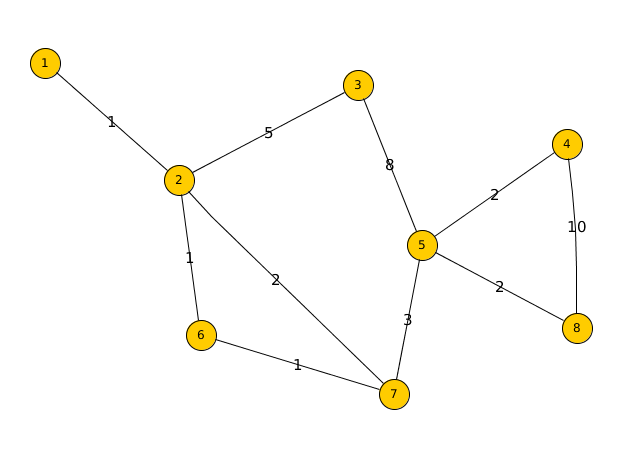
\includegraphics[scale=1]{imagenes/ej2.png}
		\caption{Instancia 1}
		\end{figure}
		
\begin{minipage}[t]{0.4\textwidth}
\begin{Verbatim}[frame=single,framesep=1cm,label= Ejemplo de entrada: instancia 1]
8 10 3
1 2 1
2 6 1
2 3 5
2 7 2
6 7 1
7 5 3
3 5 8
5 4 2
5 8 2
4 8 10
\end{Verbatim}
\end{minipage}
\hfill
\begin{minipage}[t]{0.4\textwidth}
\begin{Verbatim}[frame=single,framesep=1cm,label= Ejemplo de salida: instancia 1]
1 1 2 3 1 3 1 2
\end{Verbatim}
\end{minipage}
		
		En el ejemplo, primero el algoritmo ordena los nodos del grafo $G$ según el peso de sus máximas
		aristas. Es decir con el orden: 1 6 7 2 3 5 4 8 (en caso de empate, ordena según la suma de las aristas
		incidentes a los nodos). Luego, recorre esta lista de nodos y los va agregando de a uno al conjunto que
		dicho nodo agrega menos peso. Por ejemplo, primero agrega los nodos 1 y 6 al conjunto 1, y luego como el
		nodo 7 agrega 2 unidades de peso al conjunto 1 pero 0 al 2 (porque el conjunto 2 todavía no tiene ningún
		nodo), entonces agregamos el nodo 7 al conjunto 2. Con un razonamiento similar, en el próximo paso asignamos
		el nodo 2 al conjunto 3. De esta forma, se llega a la asignación de conjuntos 1 1 2 3 1 3 1 2 a cada uno de
		los nodos del grafo.
		
		\item Calcular el orden de complejidad de peor caso del algoritmo:
		
		Como se puede observar en el pseudocódigo que expusimos en 1.b), el algoritmo que desarrollamos utiliza dos $for$, 
		que van uno entre $1 \dots n$ y otro entre $1..k$.
		Si la complejidad de lo que hay adentro de estos ciclos es $O(T(n))$, entonces la complejidad total
		del algoritmo sería $O(knT(n))$. \\
		Dentro de estos ciclos lo que hacemos es llamar a la función CalcularHazard. Como se puede ver en el pseudocódigo
		expuesto a continuación, lo que hace dicha función es
		recorrer para el $nodoActual$ todos sus adyacentes e ir chequeando si cada adyacente está en el conjunto $conj$. 
		Si sí lo está, entonces actualizamos el hazard que generaría agregar al nodo $nodoActual$ al conjunto $conj$. 
		Esto lo hacemos de forma lineal 
		en $|V(G)|$, a partir de haber guardado el grafo $G$ en una estructura conveniente (lista de adyacencia 
		de nodos). Luego, $T(n) = O(n)$. \\
		Entonces, la complejidad de nuestro algoritmo en el peor caso es $ O(knT(n)) = O(k n^2)$.
		
		\begin{algorithm}[H]
		\SetKwInOut{Input}{input}
		\SetKwInOut{Output}{output}
		  \Input{grafo ($G$), conjunto al que quiero agregar un nodo ($conj$), nodo que quiero agregar a conj ($nodoNuevo$)}
		  \Output{costo de agregar el nodo $nodoNuevo$ al conjunto $conj$}
		  hazardAgregado = 0 \\
		  \For{cada nodo $i$ adyacente a $nodoNuevo$}{
			\If{el i-ésimo nodo adyacente a $nodoNuevo$ está en el conjunto $conj$}{
				deltaPeso = peso de la arista que une $nodoNuevo$ con el i-ésimo nodo adyacente a $nodoNuevo$ \\
				hazardAgregado = hazardAgregado + deltaPeso \\
			}
		  }
		  return hazardAgregado \\
		\caption {Función CalcularHazard, que calcula el costo de agregar el nodo $nodoNuevo$ al conjunto $conj$.}
		\end{algorithm}
		
		
		\item Describir instancias de $k$-PMP para las cuales la heurística no proporciona una solución
		óptima. Indicar qué tan mala puede ser la solución respecto de la solución óptima.
		
		Veamos dos ejemplos en los que nuestra heurística no funciona correctamente. En estos ejemplos,
		la solución es infinitamente peor que la óptima.
		
		En el primer ejemplo, se busca una 2-PMP del grafo $G_{0}$. Dicho grafo es un ciclo de nodos unidos por aristas 
		de peso infinito y con algunas aristas internas, de peso 1. Como se puede observar en los esquemas,
		la heurística proporciona una solución de peso infinito, mientras que la solución óptima tiene peso cero.
		El problema con el que se encuentra la heurística radica en que se recorren los nodos en cierto orden, y
		una vez que se coloca cada nodo en algún conjunto, este no puede ser cambiado a otro. En este 
		ejemplo en particular, se recorren los nodos del grafo en el orden: N6, N4, N2, N3, N1, N5. Entonces,
		cuando llegamos a agregar el nodo N3, ya se han agregado los nodos N6 y N2 al conjunto A, y el nodo
		N4 al conjunto B. Entonces, a esta altura ya sea que  agreguemos el nodo N3 al conjunto A o al B, en 
		cualquiera de los conjuntos agregaremos hazard infinito.
		
		\begin{figure}[H]
			\begin{minipage}{.6\textwidth}
			\centering
			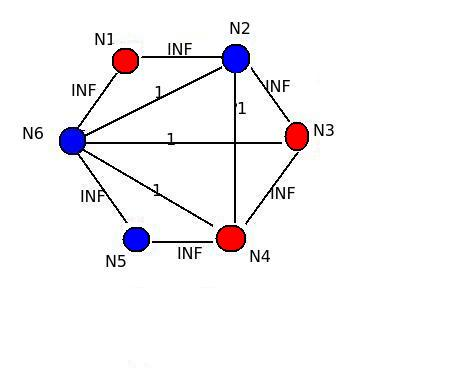
\includegraphics[width=.8\linewidth]{imagenes/ej3_11}
			\caption{Solución de la heurística}
			\end{minipage}
			\begin{minipage}{.6\textwidth}
			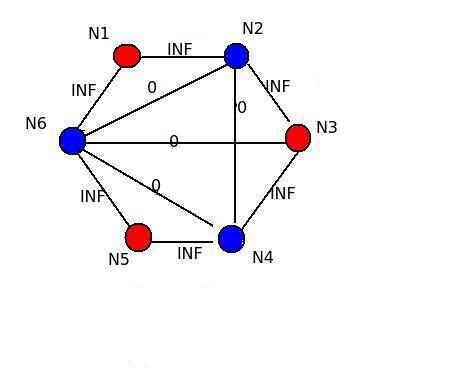
\includegraphics[width=.8\linewidth]{imagenes/ej3_12}
			\caption{Solución óptima}
			\end{minipage}
		\end{figure}
		
		
		En el ejemplo 2, se busca una 2-PMP del grafo $G_{1}$.  Dicho grafo es completo bipartito,
		a excepción de dos nodos $u$ y $v$ en uno de los conjuntos que conforman la bipartición, que están unidos por una
		arista de peso 1. Las aristas que unen cada nodo de un lado de la bipartición con nodos del otro lado de la 
		bipartición tienen, como se observa en el dibujo, peso INF. 
		La solución óptima a este problema es la presentada en la segunda
		figura, y es de peso $1 < \infty$, mientras que la solución que brinda nuestra heurística es de peso
		infinito, y una posible representación de la misma esta esquematizada en la primera figura. 
		La heurística falla
		porque vamos agregando los nodos a cada conjunto en un orden que nos conduce a una solución no óptima. En este caso,
		los nodos $u$ y $v$ son los que primero van a ser agregados a conjuntos. Entonces, como nuestro algoritmo
		es goloso y cada vez que agrega un nodo a un conjunto, lo agrega al conjunto que minimiza el hazard nuevo que se
		genera en la solución, se envía $u$ a un conjunto (rojo) y $v$ al otro (azul). Esto hace que, más adelante, para 
		cada nodo del conjunto B, como está unido tanto a $u$ como a $v$, 
		no importa si lo agregamos al conjunto rojo o al conjunto azul, en ambos casos el hazard extra que genera
	    es siempre INF. Esto hace que, al final, nuestra solución siempre tenga peso infinito. \\
	    
	    \begin{figure}[H]
		\begin{minipage}{.6\textwidth}
		\centering
		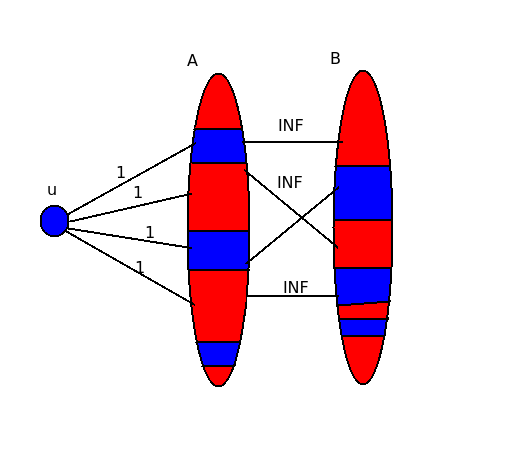
\includegraphics[width=.8\linewidth]{imagenes/ej3_21}
		\caption{Solución de la heurística}
		\end{minipage}
		\begin{minipage}{.6\textwidth}
		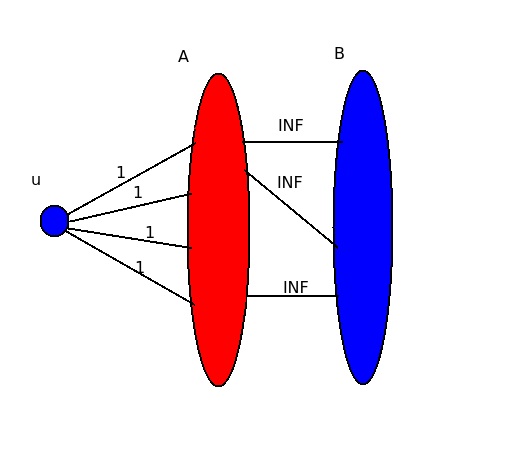
\includegraphics[width=.8\linewidth]{imagenes/ej3_22}
		\caption{Solución óptima}
		\end{minipage}
		\end{figure}
		
		
		\item Realizar una experimentación que permita observar la performance del algoritmo en términos
		de tiempo de ejecución en función del tamaño de la entrada.
		
    \end{enumerate}
    
%% =====================================================================


\newpage
\section{Problema 4} 
	
	Diseñar una heurística de búsqueda local para $k$-PMP y desarrollar los siguientes puntos:
    \begin{enumerate}
    
		\item Explicar detalladamente el algoritmo implementado. Plantear al menos dos vecindades disintas
		para la búsqueda. \\
		En el algoritmo que implementamos seguimos los siguientes pasos:
		\begin{enumerate}
			\item asignamos de forma aleatoria uno de los $k$ conjuntos a cada nodo
			\item mientras haya alguna solución vecina mejor que la actual, actualizamos todos los
			      conjuntos de nodos y el peso de la solución
			\item repetimos los dos pasos anteriores hasta que no haya una solución vecina mejor ó, hasta
			      haberlo repetido una cantidad límite de $x$ veces.
		\end{enumerate}
		
		La razón por la cual repetimos el proceso para varias soluciones iniciales es porque dependiendo
		de la solución inicial que consideremos, hallaremos un mínimo local distinto. Con lo cuál, para
		que la probabilidad de hallar el mínimo global sea lo más alta posible, hay que considerar 
		la mayor cantidad de soluciones iniciales distintas posible.
		
		Las dos vecindades que definimos fueron:
		\begin{enumerate}
			\item para cada nodo, chequear si cambiándolo a algún otro conjunto, se podría reducir el costo
			      total de la solución.
			\item para cada nodo, chequear si swappeandolo de conjunto con otro nodo ó mandándolo a un conjunto que esté
			      vacío se reduce el costo.
		\end{enumerate}
		
		A continuación, presentamos el pseudocódigo para cada una de las vecindades. \\
		\textbf{Nota: } La función calcularCosto(G,v,i) recorre los nodos adyacentes al nodo $i$, y acumula la suma
	         		    de las aristas que unen a $i$ con algún otro nodo adyacente a $i$ en la solución actual.
      \begin{algorithm}[H]
			\SetKwInOut{Input}{input}
			\SetKwInOut{Output}{output}
			  \Input{grafo $G$, solución parcial $v$}
			  \Output{modifica $v$ y genera una nueva solución parcial, $v'$}
			  
			  \For{cada nodo $i = 1 \dots n$}{
				\For{$j = $ cada conjunto $1 \dots k$}{
					costoDelNodoViejo = calcularCosto($G$, $v$, $i$) \\
					$v' = $ cambiar nodo $i$ al conjunto $j$ \\
					costoDelNodoViejo = calcularCosto($G$, $v'$, $i$) \\
					\If{costoDelNodoNuevo $<$ costoDelNodoViejo}{
						$v = v'$ \\
						actualizo costo de $v$ (en $O(1)$) \\
						res = 1 \\
					}
					\If{costoDelNodoNuevo $\geq$ costoDelNodoViejo}{
						res = 0 \\
					}
				}
			  }
			  return res \\
	  \caption{Algoritmo de búsqueda local con vecindad 1}
	  \end{algorithm}
			      
		\begin{algorithm}[H]
		\SetKwInOut{Input}{input}
		\SetKwInOut{Output}{output}
		  \Input{grafo $G$, solución parcial $v$}
		  \Output{modifica $v$ y genera una nueva solución parcial, $v'$}
		  
		  \For{ cada nodo $i = 1 \dots n$ }{
			
			// Primera parte: chequear el costo generado si hacemos algún swap \\
			costoOriginal = v.second 	// costo de la solución sin hacer el swappeo\\
			
			\For{ cada nodo $j = 1 \dots n$ }{
			
				costoNodoViejo1 = calcularCosto(G,n,v,i) \\
				costoNodoViejo2 = calcularCosto(G,n,v,j) \\
				
				swap(v.first[i], v.first[j])	// swapeo los nodos de conjunto \\
				
				costoNodoNuevo1 = calcularCosto(G,n,v,i) \\
				costoNodoNuevo2 = calcularCosto(G,n,v,j) \\
				
				costoViejo = costoNodoViejo1 + costoNodoViejo2 \\
				costoNuevo = costoNodoNuevo1 + costoNodoNuevo2 \\
				
				\eIf{costoNuevo $<$ costoViejo}{
					v.second = v.second - costoViejo + costoNuevo // actualizo costo haciendo swap\\
					break // encontré swap conveniente. Dejo de buscar posibles swaps\\
				}{
					swap(v.first[i], v.first[j])	// si no encontré un swap que disminuya el costo \\
				}
				
				
			}
			
			// Segunda Parte: calcular costo generado cambiando un nodo a un conjunto vacío \\
			\If{ hay algún conjunto vacío }{	
				\For{ cada nodo $j = 1 \dots n$ }{
					\If{cambiar nodo $j$ al conjunto $conjuntoVacio$ genera menos hazard que el swap ó genera
						menos que la solución actual (si no hicimos ningún swap) }{
						- deshago el swap (sólo si habíamos hecho un swap) \\
						- mando el nodo $j$ al conjunto $conjuntoVacio$ \\
						- break // si encontramos un conjunto propicio, dejamos de buscar \\
					}
				}				
			}
		}
		\caption{Algoritmo de búsqueda local con vecindad 2}
		\end{algorithm}
		
		En el caso de la primera  y segunda vecindad, una instancia posible y su solución serían (partiendo de la solución 
		aleatoria inicial 3 3 3 3 1 2 3 3). \\

		
\begin{minipage}[t]{0.4\textwidth}
\begin{Verbatim}[frame=single,framesep=1cm,label= Ejemplo de entrada]
8 10 3
1 2 1
2 6 1
2 3 5
2 7 2
6 7 1
7 5 3
3 5 8
5 4 2
5 8 2
4 8 10
\end{Verbatim}
\end{minipage}
\hfill
\begin{minipage}[t]{0.4\textwidth}
\begin{Verbatim}[frame=single,framesep=1cm,label= Ejemplo de salida: vecindad 1]
2 1 3 2 1 2 3 3
\end{Verbatim}
\hfill
\begin{Verbatim}[frame=single,framesep=1cm,label= Ejemplo de salida: vecindad 2]
3 3 3 3 1 3 3 2
\end{Verbatim}
\end{minipage}
		
		Vale aclarar que es esperable que, para distintas vecindades, en general nos den resulados diferentes. Además, en este ejemplo
		en particular, usando la vecindad 2 obtenemos una solución muy mala (de costo total igual a 10), mientras que para la vecindad 1,
		obtenemos una solución buena (costo total igual a 0). En este ejemplo en particular, como inicialmente no hay ningún conjunto vacío,
		cuando utilizemos la vecindad 2, sólo se van a efectuar swaps de nodos entre conjuntos, y la cantidad de nodos que hay en cada conjunto
		se va a mantener invariante (si hubiera algún conjunto vacío de seguro se le agregaría un nodo a dicho conjunto, ya que al cambiar un nodo
		a un conjunto vacío, siempre se puede reducir más el costo total de la solución que haciendo un swap). \\
		
		\item Calcular el orden de complejidad temporal de peor caso de una iteración del algoritmo de búsqueda local
			  (para las vecindades planteadas). Y si es posible, dar una cota superior para la cantidad de iteraciones
			  de la heurística. 
			  
			  En el caso de la vecindad 1, el costo de cada iteración del algoritmo de búsqueda local es $O(kn^2)$ y esto
			  se deduce fácilmente del pseudocódigo presentado en el punto anterior (empleamos dos $for$, y adentro de uno
			  de estos, llamamos a una función que calcula el costo de agregar el nodo a un conjunto, cuyo costo computacional
			  es $O(n)$, pues cada nodo es adyacente como máximo a $n-1$ nodos).
			  
			  En el caso de la vecindad 2, el costo de cada iteración del algoritmo de búsqueda es $ O(n^3) $. Esto se deduce
			  del pseudocódigo presentado más arriba: el algoritmo consta de una serie de ciclos $for$, dentro de los
			  cuáles se llama a la función $calcularCosto$, que tiene complejidad temporal $O(n)$. 
			  Luego, entre las líneas 4 y 18 la complejidad es $O(n^2)$. La línea 20 tiene una complejidad de $O(k)$, pues
			  debe recorrer todos los conjuntos chequeando la cantidad de nodos que tienen. Entre las líneas 21 y 26, la 
			  complejidad es $O(n^2)$ pues se recorren los $n$ nodos en un $for$ y en cada iteración de dicho ciclo, se 
			  recalcula el hazard que tiene la nueva solución cambiando al nodo $j$ al conjunto $conjuntoVacio$ para ver si
			  hacer este cambio genera menos hazard que generaba el swap. 
			  Entonces, como todo lo recién mencionado está metido en un $for$ que recorre todos los nodos ($O(n)$), 
			  se llega a que la complejidad es $T(n) = O(n^3) + O(nk) + O(n^3) = O(n^3) $.
			  
	    \item Realizar una experimentación que permita observar la performance del algoritmo comparando los tiempos
			  de ejecución y la calidad de las soluciones obtenidas, en función de las vecindades utilizadas y elegir,
			  si es posible, la configuración que mejores resultados provea para el grupo de instancias utilizado.
    \end{enumerate}


%% =====================================================================


\newpage
\section{Problema 5}
	Utilizando las heurísticas implementadas en los puntos anteriores, diseñar e implementar un algoritmo para k-PMP que
	use la \textbf{metaheurística GRASP} y desarrollar los siguientes puntos:
	
	 \begin{enumerate}
	 
		\item Explicar detalladamente el algoritmo implementado. Plantear distintos criterios de parada y de selección de la 
			  lista de candidatos (RCL) de la heurística golosa aleatorizada.
			  
		\item Realizar una experimentación que permita observar los tiempos de ejecución y la calidad de las soluciones
			  obtenidas. Se debe experimentar variando los valores de los parámetros de la metaheurística (lista de candidatos,
			  criterios de parada, etc.) y elegir, si es posible, la configuración que mejores resultados provea para el
			  grupo de instancias utilizado.
			  
	 \end{enumerate}

%% =====================================================================


\newpage
\section{Problema 6}
	Una vez elegidos los mejores valores de configuración para cada heurística implementada (si fue posible), realizar
	una \textbf{experimentación sobre un conjunto nuevo de instancias} para observar la performance de los métodos comparando
	nuevamente la calidad de las soluciones obtenidas y los tiempos de ejecución en función del tamaño de entrada. Para
	los casos que sea posible, comparar mediante gráficos adecuados y discutir al respecto de los mismos.


%% =====================================================================

\section{Conclusiones}


\end{document}
